\graphicspath{{SelectionCriteria/Figures/}}

\chapter{Event Selection Criteria}

\section{Preselection Criteria}

When an event is analyzed, several preselection criteria are established to count a signal observed in the detector as a valid particle. This is done to be certain that the signal received is indeed from the type of the particle that is expected. In this section, the preselection criteria used in this analysis are given. The summary of the criteria mentioned in this section is presented in Table \ref{table: preselection}. 

In each event, a maximum of six jets that had a $p_{T}$ greater than 15 GeV and its absolute value of $\eta$ less than 5.0 were stored to be analyzed later. Among this list of jets, the two jets whose summed masses resulted in the greatest mass combination were stored and defined as the Di-Jet Pair. The jet with greater momentum in the Di-Jet Pair is the leading jet and the other one in the pair is the sub-leading jet. These two jets are the ones related with the VBF process. Another variable defined regarding the Di-Jet Pair was the Di-Jet mass and corresponds to the sum of the masses from the jets in the Di-Jet Pair.  

Since the $\tau$ selection is important for this analysis, it is relevant to provide a further description of the preselection criteria for the $\tau$'s in the simulated events. For starters, a jet identified as a tau is considered a valid $\tau$ if it has a transverse momentum greater than 20 GeV. Also, it was required that a valid $\tau$ should not overlap with an electron, a muon, or a jet. That is, the $\Delta R$, defined as in Equation \ref{eq: deltaR}, should not be less than 0.3. This condition guarantees that the jet identified as a $\tau$ does not overlap with other leptons or jets. Since the final state for this analysis includes two $\tau$'s, the two taus with greater $p_{T}$ are selected among a maximum of three taus stored for each event. The leading $\tau$ is the one with highest $p_{T}$ and the sub-leading $\tau$ is the one with second highest $p_{T}$.

\begin{table}
\centering
\begin{tabular}{|c|c|}
\hline
Variable & Criteria \\
\hline
$p_{T}(j)$ & $> 40$ GeV \\
$|\eta(j)|$ & $< 5$ \\ 
$p_{T}(\tau)$ & $> 20$ GeV \\
$p_{T}(j_{B})$ & $>30$ GeV \\
$\Delta R$ & $>0.3$ \\
\hline
\end{tabular}
\caption{Preselection criteria table}
\label{table: preselection}
\end{table}

\section{Variable Cut Optimization}

To determine the optimal values for some of the variables, a study of the significance through multiple cuts was performed using the relation showed in Equation \ref{eq: significance} for each cut value. The histograms analyzed were normalized to the luminosity of each process. Taking this analyses into account, the optimal cut values for the variables $\Delta \eta$ from the Di-Jet Pair and the mass from the Di-Jet Pair, $m(jj)$, was determined.

The result for the significance study for the $\Delta \eta$ from the Di-Jet Pair is shown in Figure \ref{fig: significanceDeltaEta}. The first cut value considered was 3.8, because, as mentioned earlier, it is expected that the jets from the VBF process have a big separation in $\eta$. It is clear from the plot in Figure \ref{fig: significanceDeltaEta} that the best value for the cut is 3.8. The significance for $\Delta \eta$ values greater than 3.8 tend to decrease. This is why a selection value of 3.8 for the $\Delta \eta$ of the Di-Jet Pair was established.

\begin{figure}[H]
\centering
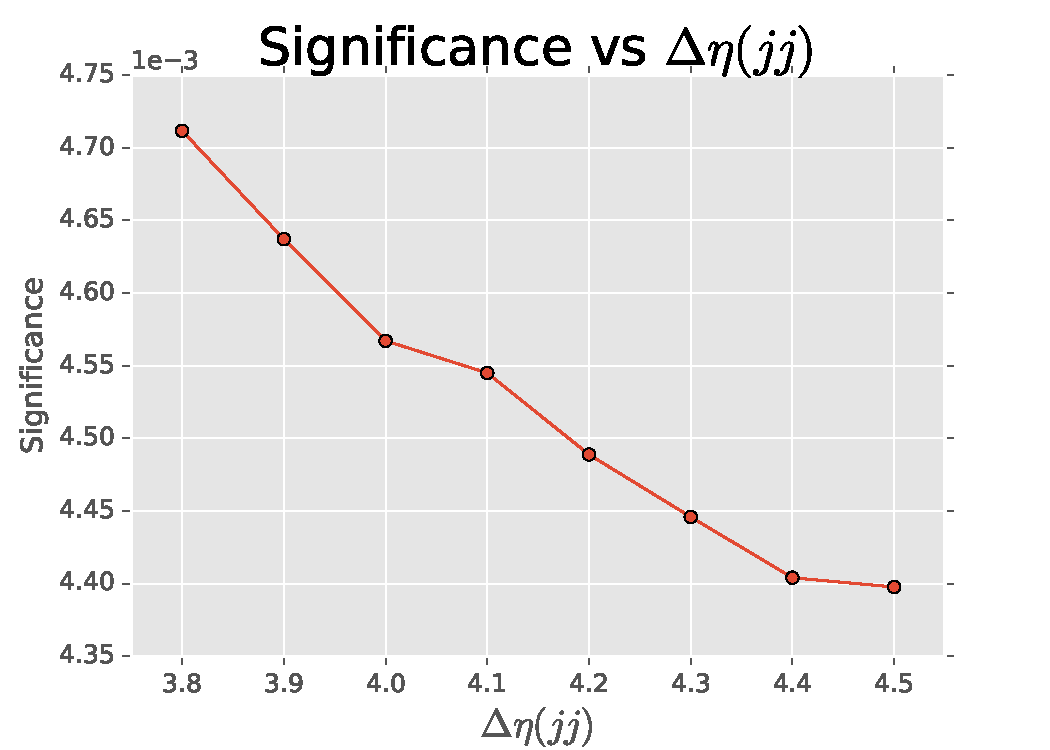
\includegraphics[width = \linewidth]{significance_deltaEta.pdf}
\caption{Significance of multiple cuts in $\Delta \eta$ diJet variable}
\label{fig: significanceDeltaEta}
\end{figure}

The other variable analyzed using the figure of significance was the total mass of the Di-Jet Pair or $m(jj)$. The result of the significance is shown in Figure \ref{fig: significanceMass}. It can be seen that the significance increases when the value for the cut in $m(jj)$ increases. 

\begin{figure}[H]
\centering
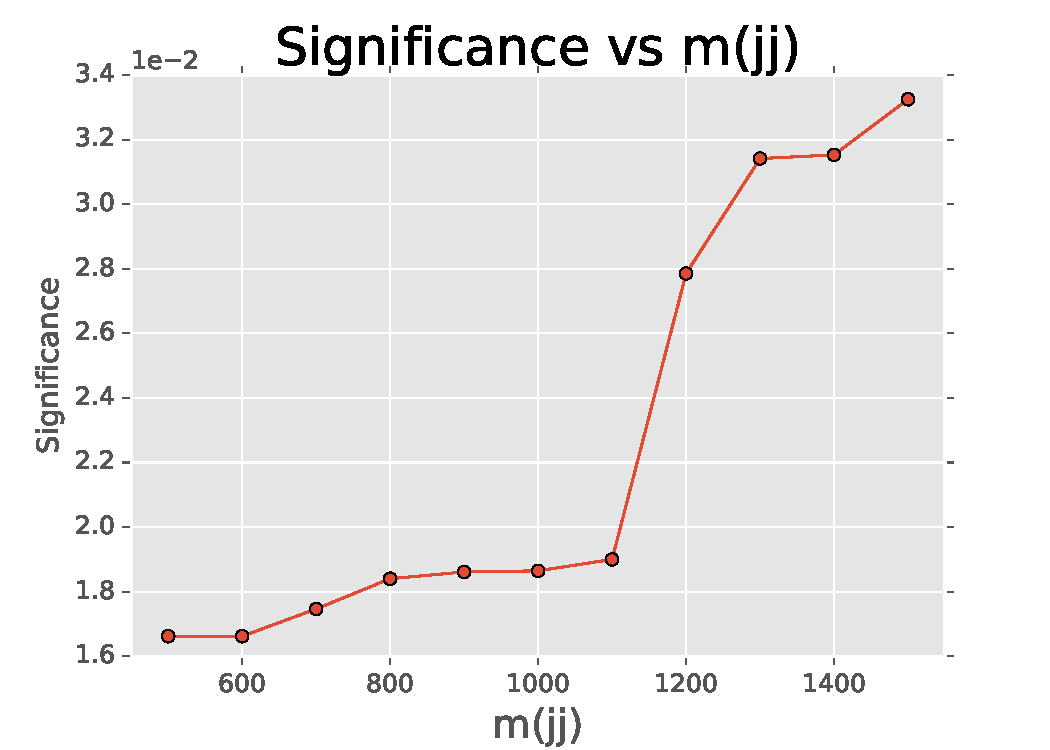
\includegraphics[width = \linewidth]{significance_mass.pdf}
\caption{Significance of multiple cuts in $m(jj)$}
\label{fig: significanceMass}
\end{figure}


\section{Event Selection Criteria}\label{sec: selectionCriteria}

In order to achieve a separation between background and signal, several successive requirements for the variables of the particles in the event were made. These requirements are defined as cuts, and for each cut the events that do not comply with the established condition are not taken into account to fill the histograms. Eight cuts were made to the histograms, storing in each cut the resulting distributions to analyze them later. The first four cuts were related with jets and $\tau$'s in the event, and the subsequent four were related with the VBF topology. In the next paragraphs of this section a description of each one of the cuts is given as well as the order in which they were performed. A summary of the selection criteria can be found in Table \ref{table: cuts}.

The first cuts that were made to the histograms were to require that the leading and sub-leading $\tau$'s should have a minimum transverse momentum of 20 GeV and a maximum of 2.1 for the absolute value of $\eta$. The latter guarantees that the $\tau$'s left are detected by the barrel and not the end-caps of the detector. That is an important condition because the detection components, such as the tracker, are in the barrel section and are more accurate than the ones in the end-caps. As a result, a signal detected in the barrel is most certain to be accurate than one detected in an end-cap.  

The next cut requires that the event does not have any B-jet. This cut is justified by the fact that one of the main backgrounds for the signal is the top anti-top ($t\bar{t}$) process. The interaction bewteen the top and anti-top quark is related with the production of jets associated with the $b$ quark or B-jets. That is why, much of the $t\bar{t}$ should be eliminated by requiring no B-jets in the event. This fact will be later analized further in chapter \ref{sec: disanalysis}. The cut that follows the one regarding the B-jets selects the events that have a minimum of two jets with transverse momentum greater than 30 GeV. This two jets must be different from the ones used in the Di-Jet Pair and are the ones that should result from the fragmentation of the quarks resulting of the W decay shown in Figure \ref{fig: HN_DY}.

The last three cuts made to the histograms are related to the VBF topology. The first of the three selects events in which the product of $\eta$ from the leading and sub-leading jets is negative. This condition guarantees that the jets in the Di-Jet Pair are in opposite hemispheres. The next cut requires that the leading and sub-leading jets of the event have a $\Delta \eta$ greater than 3.8. Finally, the last cut requires that the Di-Jet mass of the event is greater than 500 GeV.

\begin{table}
\centering
\begin{tabular}{|c|c|}
\hline
Variable & Criteria \\
\hline
$p_{T}(\tau)$ & $> 20$ GeV \\
$|\eta(\tau)|$ & $< 2.1$ \\ 
$\slashed{E}_{T}$ & $> 30$ GeV \\
Number of B-jets & $= 0$ \\
Number of jets & $ >= 2$ \\
$\eta(j_{l}) \times \eta(j_{s})$ & $<0$ \\
$\Delta \eta(jj)$ & $ > 3.8$ \\
$m(jj)$ & $> 500$ GeV \\
\hline
\end{tabular}
\caption{Selection criteria table}
\label{table: cuts}
\end{table}
